% !TEX program = xelatex
\documentclass[aspectratio=169]{beamer}
\usepackage{amsmath}
\usepackage{amssymb}
\usepackage{graphicx}
\usepackage{tcolorbox}
\usepackage{booktabs}
\usepackage{colortbl}
\usepackage{xcolor}
\usepackage{tikz}
\usetikzlibrary{angles,quotes}
\usepackage[utf8]{inputenc}

% Custom colors
\definecolor{primary}{RGB}{41, 128, 185}
\definecolor{secondary}{RGB}{52, 152, 219}
\definecolor{accent}{RGB}{231, 76, 60}
\definecolor{lightgray}{RGB}{236, 240, 241}

% Theme customization
\usetheme{Madrid}
\usecolortheme{whale}
\setbeamercolor{structure}{fg=primary}
\setbeamercolor{background canvas}{bg=white}
\setbeamercolor{normal text}{fg=black}

% Title page info
\title{Pre-Calculus 11}
\subtitle{Chapter 6.6: Absolute Values and Reciprocal Functions Summary / 絕對值與倒數函數總結}
\author{Created by Yi-Chen Lin}
\date{\today}

\begin{document}

% Title Page
\begin{frame}
    \titlepage
\end{frame}

% Overview
\begin{frame}{Chapter 6.6 Overview / 本章總覽}
    \begin{tcolorbox}[colback=lightgray,colframe=primary,title=Topics Covered]
        \footnotesize
        \begin{itemize}
            \item 6.1 Basics with Absolute Values
            \item 6.2 Absolute Value Functions
            \item 6.3 Solving Absolute Value Equations
            \item 6.4 Reciprocal Functions
            \item 6.5 Solving Equations with Two Absolute Values
        \end{itemize}
    \end{tcolorbox}
\end{frame}

% 6.1 Basics with Absolute Values
\begin{frame}{6.1 Basics with Absolute Values / 絕對值基礎}
    \begin{tcolorbox}[colback=lightgray,colframe=primary,title=Key Points]
        \footnotesize
        \begin{itemize}
            \item $|x| = \begin{cases} x, & \text{if } x \geq 0 \\ -x, & \text{if } x < 0 \end{cases}$
            \item $|x| = \sqrt{x^2}$
            \item Distance from zero on number line
            \item Always non-negative
        \end{itemize}
    \end{tcolorbox}
    \vspace{0.5em}
    \begin{center}
    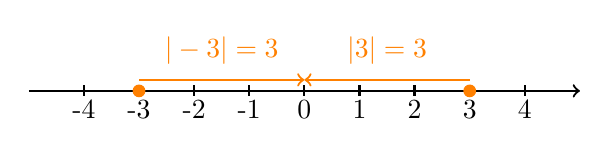
\begin{tikzpicture}[scale=0.7]
        \draw[->,thick] (-5,0) -- (5,0);
        \foreach \x in {-4,-3,-2,-1,0,1,2,3,4} {
            \draw[thick] (\x,0.1) -- (\x,-0.1);
            \node[below] at (\x,0) {\x};
        }
        \filldraw[orange] (-3,0) circle (3pt);
        \filldraw[orange] (3,0) circle (3pt);
        \draw[thick,orange,->] (-3,0.2) -- (0,0.2);
        \draw[thick,orange,->] (3,0.2) -- (0,0.2);
        \node[above,orange] at (-1.5,0.3) {$|-3|=3$};
        \node[above,orange] at (1.5,0.3) {$|3|=3$};
    \end{tikzpicture}
    \end{center}
\end{frame}

% 6.1 Practice
\begin{frame}{6.1 Practice Problems / 練習題}
    \begin{tcolorbox}[colback=lightgray,colframe=accent,title=Practice]
        \footnotesize
        \begin{enumerate}
            \item Evaluate $|25 - 17|$
            \item Solve $|x+5| = 12$
            \item Solve $|2x-4| = 9$
            \item Order from least to greatest: $|-7.5|, |-8.2|, |-3.4|$
        \end{enumerate}
    \end{tcolorbox}
\end{frame}

\begin{frame}{6.1 Solutions / 解答}
    \begin{tcolorbox}[colback=lightgray,colframe=accent,title=Solutions]
        \footnotesize
        \begin{enumerate}
            \item $|25 - 17| = |8| = 8$
            \item $x+5 = 12$ or $x+5 = -12$; $x = 7$ or $x = -17$
            \item $2x-4 = 9$ or $2x-4 = -9$; $x = 6.5$ or $x = -2.5$
            \item $|-3.4|, |-7.5|, |-8.2|$ (3.4, 7.5, 8.2)
        \end{enumerate}
    \end{tcolorbox}
\end{frame}

% 6.2 Absolute Value Functions
\begin{frame}{6.2 Absolute Value Functions / 絕對值函數}
    \begin{tcolorbox}[colback=lightgray,colframe=primary,title=Key Points]
        \footnotesize
        \begin{itemize}
            \item $y = |f(x)|$ reflects negative parts above $x$-axis
            \item Piecewise definition: $y = \begin{cases} f(x), & f(x) \geq 0 \\ -f(x), & f(x) < 0 \end{cases}$
            \item Find $x$-intercepts to determine reflection points
        \end{itemize}
    \end{tcolorbox}
    \vspace{0.5em}
    \begin{center}
    \begin{tikzpicture}[scale=0.6]
        \draw[->] (-2,0) -- (4,0) node[right] {$x$};
        \draw[->] (0,-1) -- (0,3) node[above] {$y$};
        \draw[thick,blue] (1,0) -- (3,2);
        \draw[thick,blue] (1,0) -- (-1,2);
        \node[below] at (1,0) {1};
        \node[right] at (3,2) {$y = |x-1|$};
    \end{tikzpicture}
    \end{center}
\end{frame}

% 6.2 Practice
\begin{frame}{6.2 Practice Problems / 練習題}
    \begin{tcolorbox}[colback=lightgray,colframe=accent,title=Practice]
        \footnotesize
        \begin{enumerate}
            \item Graph $y = |x^2 - 4|$
            \item Write piecewise form for $y = |x + 2|$
            \item Find $x$-intercepts of $y = |x^2 - 9|$
            \item Graph $y = |x^3 - x|$
        \end{enumerate}
    \end{tcolorbox}
\end{frame}

\begin{frame}{6.2 Solutions / 解答}
    \begin{tcolorbox}[colback=lightgray,colframe=accent,title=Solutions]
        \footnotesize
        \begin{enumerate}
            \item V-shape with vertex at $(0,4)$, $x$-intercepts at $x = \pm 2$
            \item $y = \begin{cases} x+2, & x \geq -2 \\ -(x+2), & x < -2 \end{cases}$
            \item $x = \pm 3$ (where $x^2 - 9 = 0$)
            \item Reflects negative parts of $y = x^3 - x$ above $x$-axis
        \end{enumerate}
    \end{tcolorbox}
\end{frame}

% 6.3 Solving Absolute Value Equations
\begin{frame}{6.3 Solving Absolute Value Equations / 解絕對值方程式}
    \begin{tcolorbox}[colback=lightgray,colframe=primary,title=Key Points]
        \footnotesize
        \begin{itemize}
            \item For $|x| = a$, set up two cases: $x = a$ and $x = -a$
            \item Always check for extraneous roots
            \item $|x| = -a$ has no solution if $a > 0$
        \end{itemize}
    \end{tcolorbox}
    \vspace{0.5em}
    \begin{center}
    \textbf{Example:} $|x-3| = 7$\\
    $x-3 = 7$ or $x-3 = -7$\\
    $x = 10$ or $x = -4$
    \end{center}
\end{frame}

% 6.3 Practice
\begin{frame}{6.3 Practice Problems / 練習題}
    \begin{tcolorbox}[colback=lightgray,colframe=accent,title=Practice]
        \footnotesize
        \begin{enumerate}
            \item Solve $|x-1| = x+1$
            \item Solve $|2x-5| = |x+4|$
            \item Solve $|x^2-6x+8| = 2$
            \item Which has no solution: $|x+3| = -5$ or $|x+3| = 5$?
        \end{enumerate}
    \end{tcolorbox}
\end{frame}

\begin{frame}{6.3 Solutions / 解答}
    \begin{tcolorbox}[colback=lightgray,colframe=accent,title=Solutions]
        \footnotesize
        \begin{enumerate}
            \item Case 1: $x-1 = x+1$ (no solution); Case 2: $x-1 = -(x+1)$; $x = 0$
            \item $x = 9$ or $x = \frac{1}{3}$
            \item $x = 3 \pm \sqrt{3}$
            \item $|x+3| = -5$ has no solution (absolute value cannot be negative)
        \end{enumerate}
    \end{tcolorbox}
\end{frame}

% 6.4 Reciprocal Functions
\begin{frame}{6.4 Reciprocal Functions / 倒數函數}
    \begin{tcolorbox}[colback=lightgray,colframe=primary,title=Key Points]
        \footnotesize
        \begin{itemize}
            \item $y = \frac{1}{f(x)}$
            \item Vertical asymptotes where $f(x) = 0$
            \item Invariant points where $f(x) = \pm 1$
            \item Horizontal asymptote usually $y = 0$
        \end{itemize}
    \end{tcolorbox}
    \vspace{0.5em}
    \begin{center}
    \begin{tikzpicture}[scale=0.6]
        \draw[->] (-2,0) -- (4,0) node[right] {$x$};
        \draw[->] (0,-2) -- (0,3) node[above] {$y$};
        \draw[thick,red,dashed] (1,-2) -- (1,3) node[above] {VA};
        \draw[thick,blue,domain=0.5:0.8] plot (\x,{1/(\x-1)});
        \draw[thick,blue,domain=1.2:3] plot (\x,{1/(\x-1)});
        \node[right] at (3,0.5) {$y = \frac{1}{x-1}$};
    \end{tikzpicture}
    \end{center}
\end{frame}

% 6.4 Practice
\begin{frame}{6.4 Practice Problems / 練習題}
    \begin{tcolorbox}[colback=lightgray,colframe=accent,title=Practice]
        \footnotesize
        \begin{enumerate}
            \item Find vertical asymptotes of $y = \frac{1}{x^2-4}$
            \item Find invariant points of $y = \frac{1}{x+2}$
            \item Graph $y = \frac{1}{x^2}$
            \item Domain of $y = \frac{1}{\sqrt{x-3}}$?
        \end{enumerate}
    \end{tcolorbox}
\end{frame}

\begin{frame}{6.4 Solutions / 解答}
    \begin{tcolorbox}[colback=lightgray,colframe=accent,title=Solutions]
        \footnotesize
        \begin{enumerate}
            \item $x = \pm 2$ (where $x^2-4 = 0$)
            \item $x = -1$ and $x = -3$ (where $x+2 = \pm 1$)
            \item Hyperbola with VA at $x = 0$, HA at $y = 0$
            \item $x > 3$ (to avoid division by zero and negative under square root)
        \end{enumerate}
    \end{tcolorbox}
\end{frame}

% 6.5 Solving Equations with Two Absolute Values
\begin{frame}{6.5 Solving Equations with Two Absolute Values / 解含兩個絕對值的方程式}
    \begin{tcolorbox}[colback=lightgray,colframe=primary,title=Key Points]
        \footnotesize
        \begin{itemize}
            \item Consider all possible sign combinations (4 cases)
            \item Use number line to determine valid intervals
            \item Always check solutions for extraneous roots
        \end{itemize}
    \end{tcolorbox}
    \vspace{0.5em}
    \begin{center}
    \textbf{Example:} $|x-2| + |x+6| = 11$\\
    Cases: $x \geq 2$, $-6 \leq x < 2$, $x < -6$\\
    Solutions: $x = 3.5$, $x = -7.5$
    \end{center}
\end{frame}

% 6.5 Practice
\begin{frame}{6.5 Practice Problems / 練習題}
    \begin{tcolorbox}[colback=lightgray,colframe=accent,title=Practice]
        \footnotesize
        \begin{enumerate}
            \item Solve $|x-1| + |x+5| = 8$
            \item Solve $|x+3| - |x-2| = 4$
            \item Solve $|x-4| + |x+2| = 10$
            \item How many cases for $|x-a| + |x-b| = c$?
        \end{enumerate}
    \end{tcolorbox}
\end{frame}

\begin{frame}{6.5 Solutions / 解答}
    \begin{tcolorbox}[colback=lightgray,colframe=accent,title=Solutions]
        \footnotesize
        \begin{enumerate}
            \item $x = 2$ and $x = -6$
            \item $x = 1.5$ (only valid solution)
            \item $x = 6$ and $x = -4$
            \item 3 cases: $x \geq \max(a,b)$, $\min(a,b) \leq x < \max(a,b)$, $x < \min(a,b)$
        \end{enumerate}
    \end{tcolorbox}
\end{frame}

% Final Review Questions
\begin{frame}{Final Review Questions / 綜合練習}
    \begin{tcolorbox}[colback=lightgray,colframe=primary,title=Comprehensive Review]
        \footnotesize
        \begin{enumerate}
            \item Evaluate $|-15| + |7|$
            \item Solve $|2x-3| = 7$
            \item Graph $y = |x^2 - 1|$
            \item Find asymptotes of $y = \frac{1}{x^2-9}$
            \item Solve $|x-3| + |x+1| = 6$
            \item Explain the difference between $|f(x)|$ and $\frac{1}{f(x)}$
        \end{enumerate}
    \end{tcolorbox}
\end{frame}

\begin{frame}{Final Review Solutions / 綜合練習解答}
    \begin{tcolorbox}[colback=lightgray,colframe=accent,title=Solutions]
        \footnotesize
        \begin{enumerate}
            \item $|-15| + |7| = 15 + 7 = 22$
            \item $2x-3 = 7$ or $2x-3 = -7$; $x = 5$ or $x = -2$
            \item V-shape with vertex at $(0,1)$, $x$-intercepts at $x = \pm 1$
            \item Vertical asymptotes: $x = \pm 3$; Horizontal asymptote: $y = 0$
            \item $x = 4$ and $x = -2$
            \item $|f(x)|$ reflects negative parts above $x$-axis; $\frac{1}{f(x)}$ creates reciprocal with asymptotes
        \end{enumerate}
    \end{tcolorbox}
\end{frame}

\end{document} 